\chapter{Results}
\label{results}

While working and using the RMT toll, many limitations were found and described in \cref{subsub-limitation}. A new internal and external architecture was proposed that focuses on solving those problems; these modifications will allow the system to scale better, provide better performance, and make it easy to use by accessing the tool in the browser.

The \cref{sec-cloud} explains the cloud solution of the new RMT architecture; \cref{sub-async} discusses the methodologies for implementing asynchronous operations within the tool; \cref{sub-tests} explaining about applying tests on the RMT; \cref{sec-closingproposal} comments about the closing remarks

\section{Archtecure \& Cloud Technologies}

The technologies selected for the revised architecture were thought to take greater advantage of what the cloud offers. 

Two technologies were selected for storage: the S3 Bucket from AWS and the Redis deployed as serverless with the Elasticache service. The S3 is a cheap object storage provided by AWS that is scalable and has a 99.9\% monthly uptime; it allows the tool to save zip files for each project and to be re-retrieved afterward \cite{S3}. The Redis is a memory database and is widely used for caching and allows us to easily save the project state \cite{Redis}.

The Simple Service Queue (SQS), a fully managed serverless queue service developed by AWS, was chosen for microservice communication. The SQS offers an async queue communication, having an order message delivered first in, first out (FIFO), or without an order \cite{sqs}.

Two services were selected for external communication: the Elastic Load Balancer (ELB) and the Amazon API Gateway. The ELB balances the load (requests) between services with a round-robin strategy \cite{Elb}. The API Gateway allows external communication to access the functionality for the back-end microservices \cite{Gateway}.

\section{Architecture Refactoring \& Cloud Approach}
\label{sec-cloud}
The revised architecture introduces several modifications in the inter-service communication protocols. The tool initial tool version had three services and one Java desktop application. 

The revised architecture transitioned the desktop application to a web-based platform, altering each service's operational dynamics. The services were renamed to reflect a more meaningful nomenclature: the Metrics Service was redefined as the Metrics Calculator Service, the Intermediary Service was reconstituted as the Refactoring and Metrics Management Service, and the Detection Service was redesignated as the Detection and Refactoring Service. The newly devised architecture is illustrated in \Cref{fig-architecture}.

\begin{figure}[ht!]
\SetCaptionWidth{\textwidth}
\caption{RMT revised architecture diagram}
\label{fig-async}
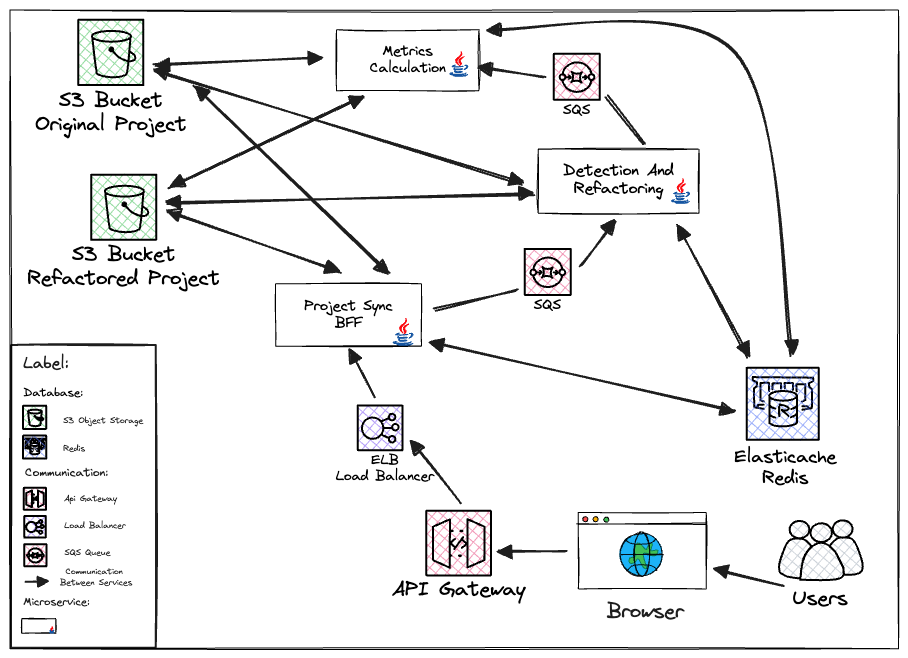
\includegraphics[width =\textwidth, scale=0.2]{Chapter-5/Figures/Async.png}
\SourceOrNote{Own authorship (2024)}
\end{figure}
\FloatBarrier

\subsection{Comunication Improvements}

The communication type was switched to queues instead of HTTP requests. The modification primarily aims to establish a communication mechanism with enhanced configurability in the event of failures, as the services must acknowledge the messages, or they will be re-tried as many times as configured. Queues also offer an asynchronous communication that is out of the box. Otherwise, in the HTTP request, the retry has to be implemented on the client side according to the server response. It is also possible to have an HTTP asynchronous request, but it also has to be implemented on the client side.

The Simple Queue Service (SQS) operates in its default configuration, implementing a quintuple retry mechanism to transmit a JSON object containing the project identifier between microservices.

\subsection{Storage \& Database Improvements}

The initial version of RMT utilizes MongoDB GridFs for file storage, a feature designed to facilitate the preservation of files within the database architecture. The updated version uses Amazon S3 for project storage, using a dual-bucket strategy: one designated for the original project and the other for the refactored iterations. All microservices are granted access to the designated buckets, enabling seamless file storage and retrieval. The project information and statuses are stored in the Redis in-memory document database, and all services also have access.

\section{Services Behaivour Improviments}
\label{sub-async}

\begin{figure}[ht!]
\SetCaptionWidth{\textwidth}
\caption{New Architecture Use Case}
\label{fig-usecasenew}
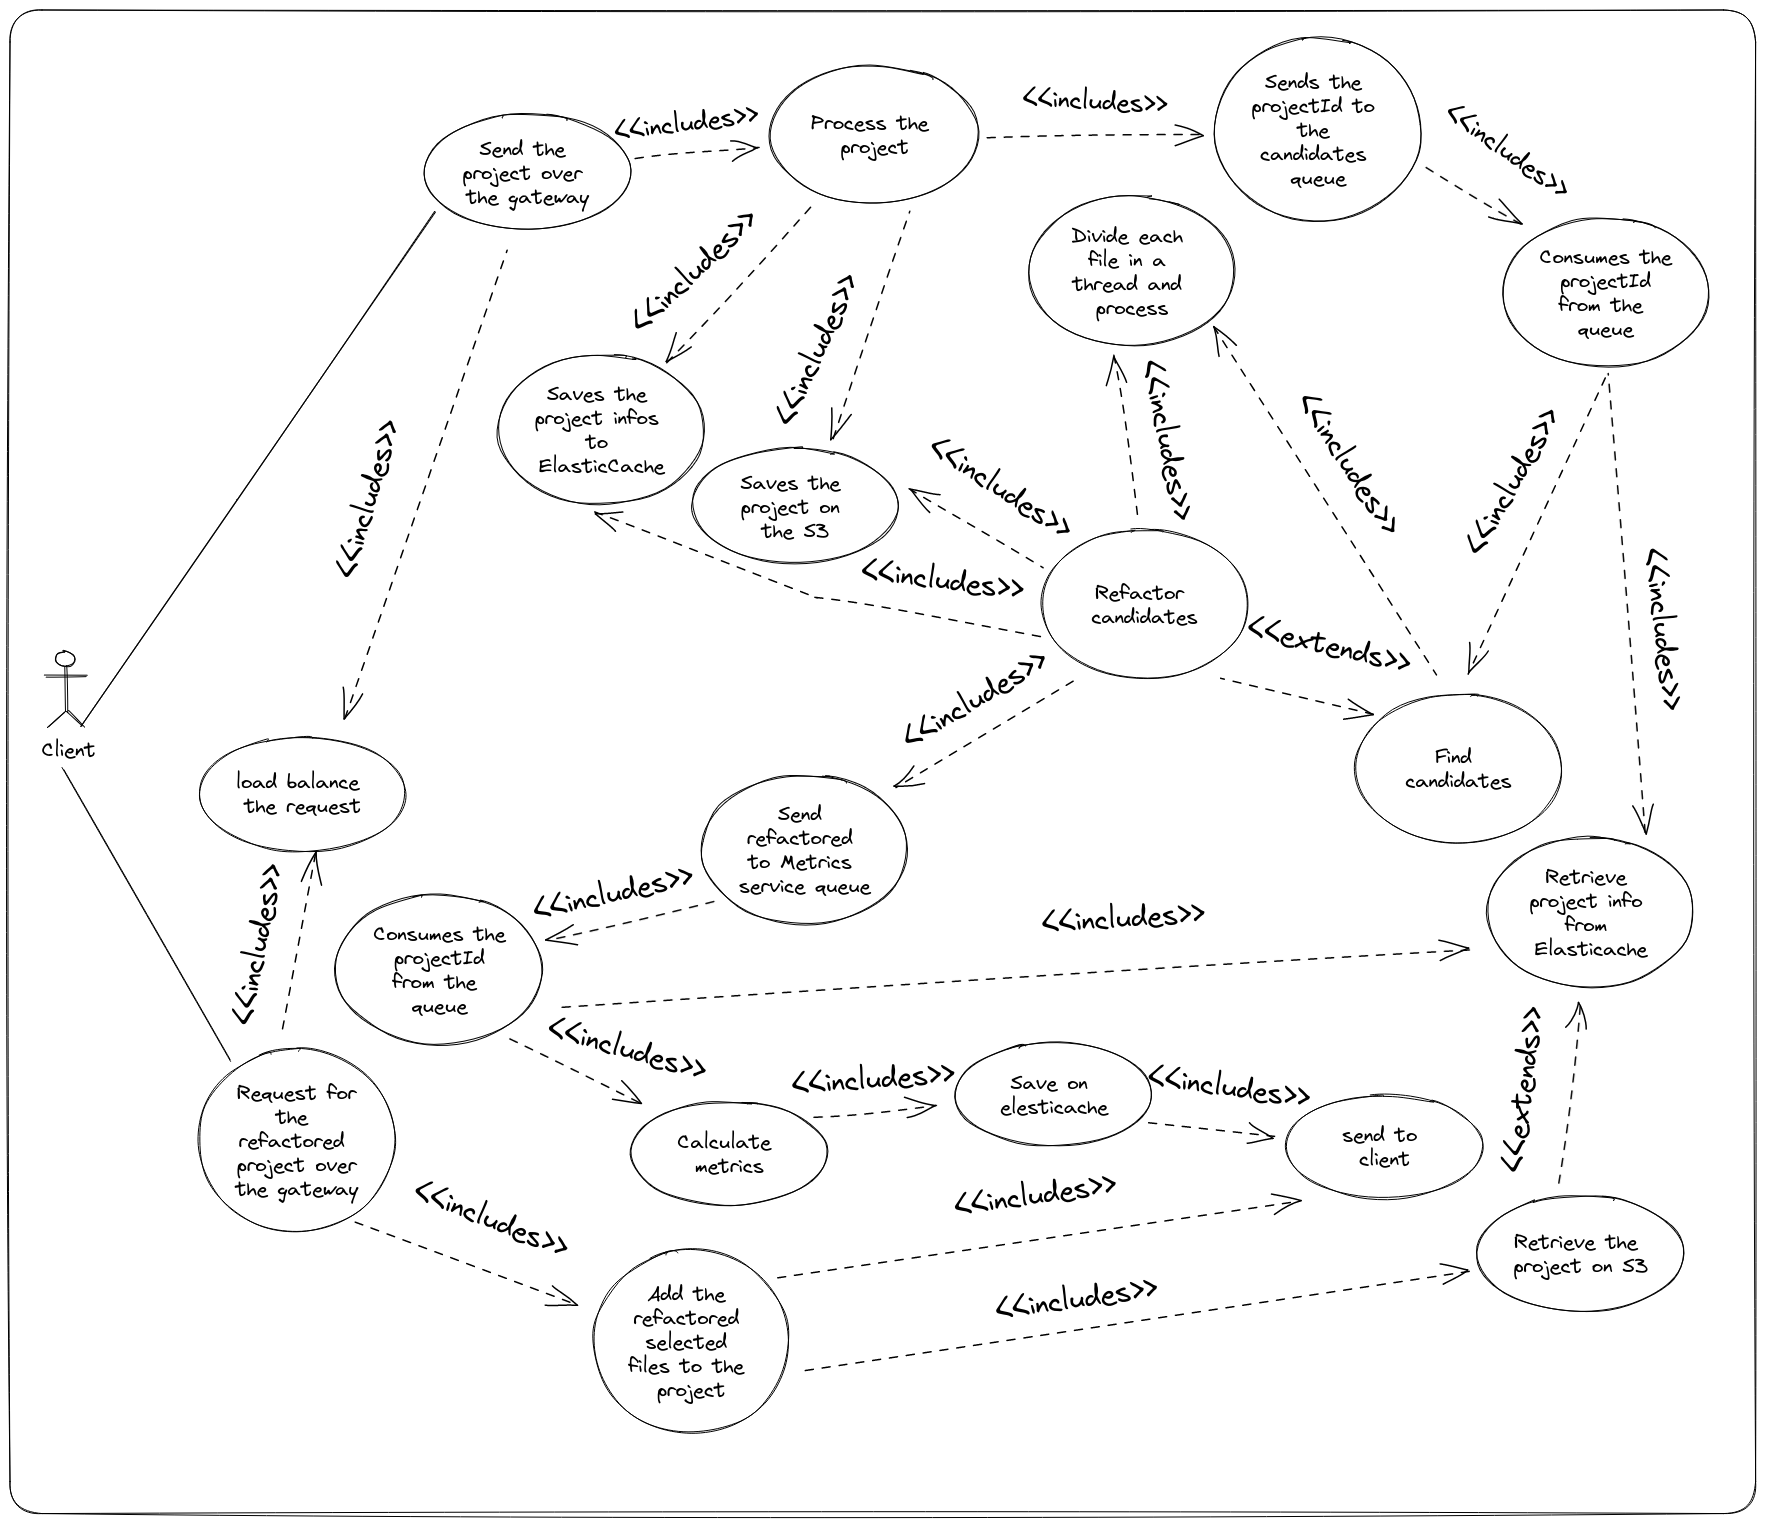
\includegraphics[width =\textwidth, scale=0.2]{Chapter-5/Figures/usecasenew.png}
\SourceOrNote{Own authorship (2023)}
\end{figure}
\FloatBarrier


The new tool flow will work as described on the \Cref{fig-async}, starting with the user selecting the project and sending it over to the API Gateway that will connect with the Intermediary Service by the ELB; the service will have one queue one for finding refactoring candidates, and then refactor it, both will send the information to the Detection Service which will process and send the information to the Metrics Service if any candidate was found. While the Detection and Metrics service is working, the Intermediary service is pulling on the Redis to see if the process is finished to send back the information to the client, which is a long pull on the intermediary service as shown on use case diagram in \Cref{fig-usecasenew}.


As seen before, the throttling is happening on the Detection Service as it does not work with threads and has too much file system access; an asynchronous approach with a controlled file system access approach can solve the problem. Making the tool work with thread will improve its performance as it can process many files simultaneously, as described in \Cref{fig-threading}.

\begin{figure}[ht!]
\SetCaptionWidth{\textwidth}
\caption{RMT multi-thread structure}
\label{fig-threading}

\includegraphics[width =\textwidth, scale=0.2]{Chapter-5/Figures/threadDivision.png}
\SourceOrNote{Own authorship (2023)}
\end{figure}

The Detection Service will access the S3 only once per operation, once to search for candidates and once to refactor to solve the problem of the file system being accessed many times to retrieve the project.

When the Detection services receive a project, it will divide the files over the JVM threads to be individually processed simultaneously and compile together after increasing the CPU usage of the service in exchange for performance. The async architecture will help to achieve more threads as it will not hold any thread connection with BFF.

\subsection{Tests implementantion}
\label{sub-tests}

As refactoring is a good practice for coding tests also are. For that reason, unit tests will be applied to the tool for every file with logic, trying to achieve a unit test coverage of 98\% with the help JUnit 5 test framework for Java and Mockito, another Java framework focused on mocking classes and methods.

Unit tests are important, but they cannot guarantee that the integration of the classes and logic is working; that is why integration tests will be implemented with Testcontainers. A framework that manipulates Docker containers to run over tests enabling the service to create a local stack of the cloud environment for tests and use, such as it would work on the production running the application locally with the programmed scenarios.



\section{Java Update \& Framework Refactoring}
\label{sec-framework}

The proposed approach intends to upgrade the RMT tool bridging it to a more modern and robust environment. The first improvement is to change the Spring boot framework, a Java framework enterprise-ready and widely used in the market according to \textcite{Mythily2022}. The framework change is supported by three main reasons described below.
\begin{itemize}
\item Java EE 8 works but has some drawbacks compared to new technologies, such as no integrated server, barriers to the developer running the tool, and losing time configuring a web server. On the other hand, Spring has a tomcat web server integrated and only needs one maven command to be ready and running.
\item Spring boot has production-ready cloud-native data, among other integrations, which reduces the programming and configuration time.
\item As the RMT is divided into services, Spring has built-in tools to manage services like the Eureka service registry. Now the management is made by the tool.
\end{itemize}

Following the framework update, an architecture change is also planned, altering the communication of the services to be async so each service would run independently and faster than the current sync architecture. To support all the new features, the infrastructure of the RMT will be based on the AWS cloud service as it provides high scalability and availability, so the user does not have to run the program on his computer.

Following the refactoring proposal, the spring boot framework will be used. The community highly supports it and has many libraries built to help its development.
The first step to upgrade the services is to change the Java version from 8 to 17, which will receive support until 2024. This change was based on new features such as better support for containers, records, and many other improvements after Java 8 release \cite{java8to17}. 

The RMT tool uses Java EE to create injection dependencies, web servers, and many other configurations; since Java 8, the ownership has changed from Oracle to Eclipse foundation, changing its imports from Javax to Jakarta EE described by \textcite{java8to17} on the oracle blog.

The Spring ecosystem will substitute the JavaEE, an open-source framework that uses the Jakarta EE implementations to work but abstracts many functionalities for the programmer. According to the \textcite{javasurvey}, Spring has up to 57\% of the market share compared with other frameworks; it's best to consider that Spring does not compete with Jakarta EE. The change is based on the spring facility to integrate with the cloud, having projects like spring cloud only to facilitate the development of cloud-native applications. These Spring data offer abstractions to communicate to databases, among others.

\section{Closing Remarks}
\label{sec-closingproposal}
The proposal of tool refactoring presented in this chapter focused on addressing several flaws identified in the RMT tool. The proposed changes involved an internal and external architecture that aims to improve the scalability, performance, and accessibility of the tool through the cloud. The RMT tool's communication changes were directed towards creating more configuration over failure, using queues over HTTP requests. 

The proposed infrastructure was deployed on the AWS cloud, and technologies can be used locally with the AWS LocalStack. The new architecture uses Fargate, Amazon SQS, AWS API Gateway, ELB, Elasticache Redis, and S3 Bucket services. 

The RMT tool's database was changed to Amazon S3 and Elasticache, with SQS substituting most of the REST calls of the tools. The Intermediary Service works only as a BFF communicating with the Detection Service. This proposal allows the RMT tool to work asynchronously, with users having to pull information on the BFF, verify the status on the Elasticache, and send information to the client when it is ready.